% Density-Based Spatial Clustering of Applications with Noise
\begin{frame}[allowframebreaks]{Clustering - Density-Based Methods}
\begin{itemize}
    \setlength{\itemsep}{0.1em}
    \item Clustering based on density (local cluster criterion), such as density-connected points or based on an explicitly constructed density function.
    \item \textbf{Major features}:
    \begin{itemize}
        \item Discover clusters of arbitrary shape
        \item Handle noise
        \item One scan
        \item Need density parameters
    \end{itemize}

    \framebreak
    
    \item \textbf{Major algorithms}:
    \begin{itemize}
        \item DBSCAN (Density-Based Spatial Clustering of Applications with Noise): Ester, et al. (KDD’96)
        \item OPTICS (Ordering Points to Identify the Clustering Structure): Ankerst, et al. (SIGMOD’99)
        \item HDBSCAN (Hierarchical Density-Based Spatial Clustering of Applications with Noise): Campello, et al. (ACM TIST’15)
        \item DENCLUE (DENsity-based CLUstEring): Hinneburg and Gabriel (KDD’97)
        \item CLIQUE (CLustering In QUEst): Karypis, Han, and Kumar (SIGMOD’98)
    \end{itemize}
\end{itemize}
\end{frame}

\begin{frame}[allowframebreaks]{Clustering - DBSCAN}
\begin{itemize}
    \item \textbf{DBSCAN} (Density-Based Spatial Clustering of Applications with Noise):
    \begin{itemize}
        \item Density = number of points within a specified radius $\epsilon$.
        \item A point is a core point if it has more than a specified number of points (MinPts) within $\epsilon$. These are points that are at the interior of a cluster.
        \item A border point has fewer than MinPts within $\epsilon$, but is in the neighborhood of a core point
        \item A noise point is any point that is not a core point or a border point.
        \item Groups together points that are closely packed together, marking as outliers points that lie alone in low-density regions.
        \item Parameters:
        \begin{itemize}
            \item $\epsilon$: Maximum distance between two points for them to be considered as in the same neighborhood.
            \item MinPts: Minimum number of points required to form a dense region.
        \end{itemize}
    \end{itemize}
\end{itemize}

\framebreak

\begin{figure}
    \centering
    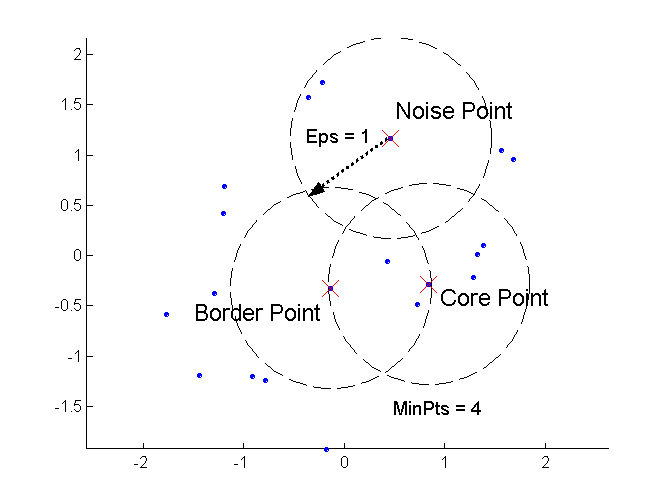
\includegraphics[width=0.95\textwidth,height=0.8\textheight,keepaspectratio]{images/dul/dbscan/dbscan-features.png}
    \caption{DBSCAN features: Core, Border, and Noise Points}
\end{figure}
\end{frame}


\begin{frame}[allowframebreaks]{Clustering - DBSCAN: Algorithm}
\begin{algorithm}[H]
\caption{Graph-Based DBSCAN Clustering}
\KwIn{Set of points $P$, distance threshold $\varepsilon$, minimum number of points $minPts$}
\KwOut{A set of clusters}

Construct a directed graph $G = (V, E)$ where each node in $V$ corresponds to a point in $P$\;

\ForEach{point $c \in P$}{
    \If{$c$ is a core point (i.e., $|\mathcal{N}_\varepsilon(c)| \geq minPts$)}{
        \ForEach{point $p \in \mathcal{N}_\varepsilon(c)$}{
            Add a directed edge $(c \rightarrow p)$ to $E$\;
        }
    }
}

$N \leftarrow V$\;

\While{there exists a core point $c \in N$}{
    Let $X$ be the set of nodes reachable from $c$ via directed edges in $G$\;
    Form a cluster $C = X \cup \{c\}$\;
    Remove all nodes in $C$ from $N$\;
}

\end{algorithm}
\end{frame}

\begin{frame}[allowframebreaks]{Clustering - DBSCAN: Core, Border, and Noise Points}
\begin{columns}
    \begin{column}{0.5\textwidth}
       \begin{figure}
            \centering
            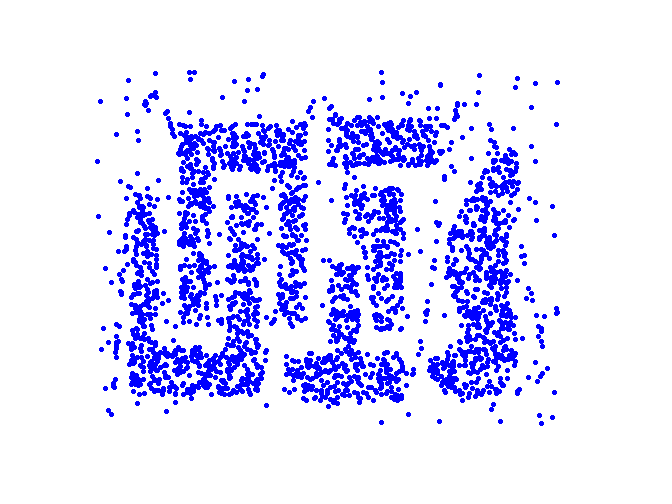
\includegraphics[width=1.2\textwidth,keepaspectratio]{images/dul/dbscan/dbscan-original-pts-1.png}
            \caption{Original Points}
        \end{figure}
    \end{column}
    \begin{column}{0.5\textwidth}
        \begin{figure}
            \centering
            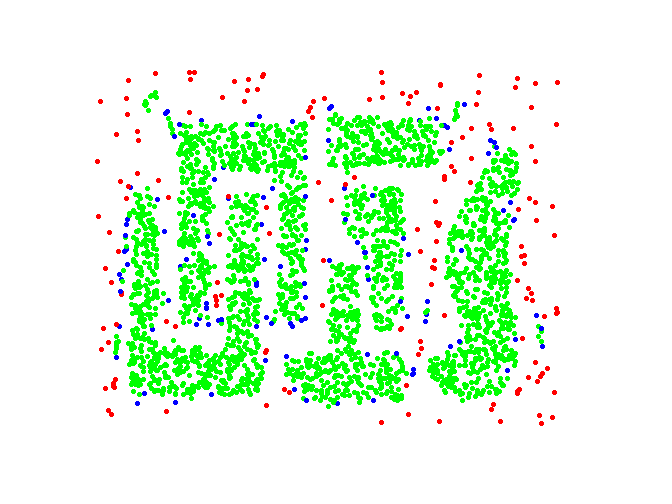
\includegraphics[width=1.2\textwidth,keepaspectratio]{images/dul/dbscan/dbscan-core-border-noise.png}
            \caption{Point types: \textcolor{green}{Core}, \textcolor{blue}{Border}, and \textcolor{red}{Noise} Points}
        \end{figure}
    \end{column}
\end{columns}

\begin{center}
Eps = 10, MinPts = 4
\end{center}

\end{frame}

\begin{frame}[allowframebreaks]{When DBSCAN Works Well}
\begin{columns}
    \begin{column}{0.5\textwidth}
       \begin{figure}
            \centering
            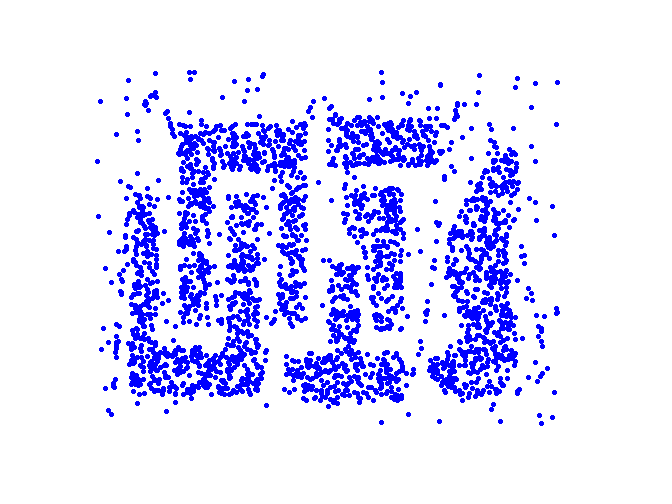
\includegraphics[width=1\textwidth,keepaspectratio]{images/dul/dbscan/dbscan-original-pts-1.png}
            \caption{Original Points}
        \end{figure}
    \end{column}
    \begin{column}{0.5\textwidth}
        \begin{figure}
            \centering
            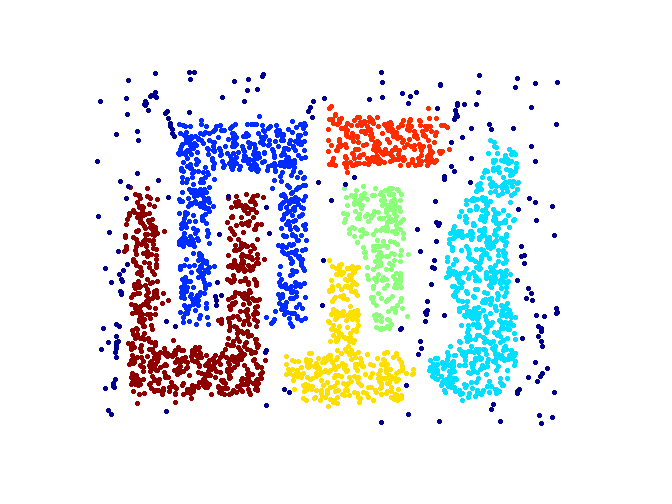
\includegraphics[width=1\textwidth,keepaspectratio]{images/dul/dbscan/dbscan-clusters.png}
            \caption{Clusters identified by DBSCAN}
        \end{figure}
    \end{column}
\end{columns}

DBSCAN works well when:
\begin{itemize}
        \item Clusters are of varying shapes and sizes.
        \item There is a clear distinction between dense and sparse regions.
        \item The data contains noise or outliers.
\end{itemize}
\end{frame}

\begin{frame}[allowframebreaks]{When DBSCAN Doesn't Works Well}
\begin{columns}
    \begin{column}{0.5\textwidth}
       \begin{figure}
            \centering
            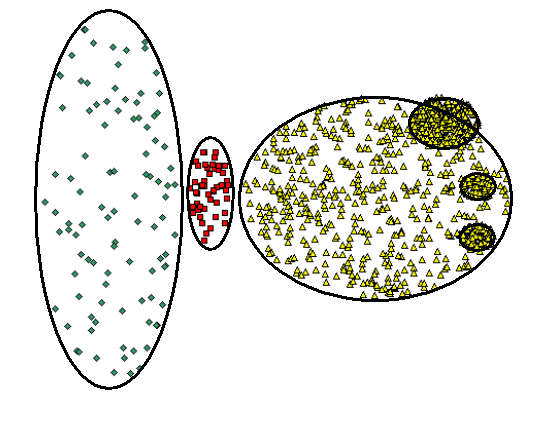
\includegraphics[width=0.9\textwidth,keepaspectratio]{images/dul/dbscan/dbscan-original-pts-2.png}
            \caption{Original Points}
        \end{figure}

        DBSCAN does not work well when:
        \begin{itemize}
            \item Clusters are of varying densities.
            \item The data has varying scales or dimensions.
            \item There are overlapping clusters.
            \item The choice of $\epsilon$ and MinPts is not suitable for the data distribution.
        \end{itemize}
    \end{column}
    \begin{column}{0.5\textwidth}
        \begin{figure}
            \centering
            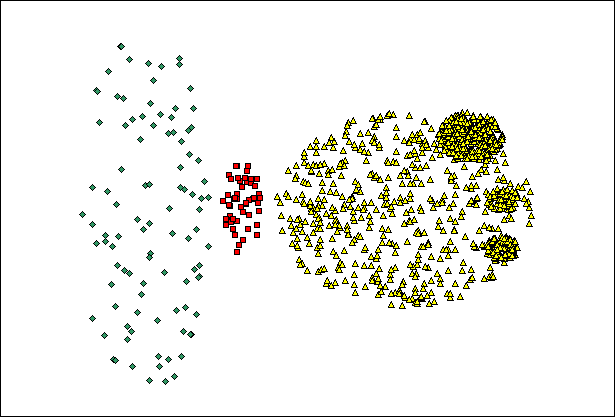
\includegraphics[width=0.9\textwidth,keepaspectratio]{images/dul/dbscan/dbscan-clusters-1.png}
            \caption{MinPts=4, $\epsilon$=9.75}
        \end{figure}
        \begin{figure}
            \centering
            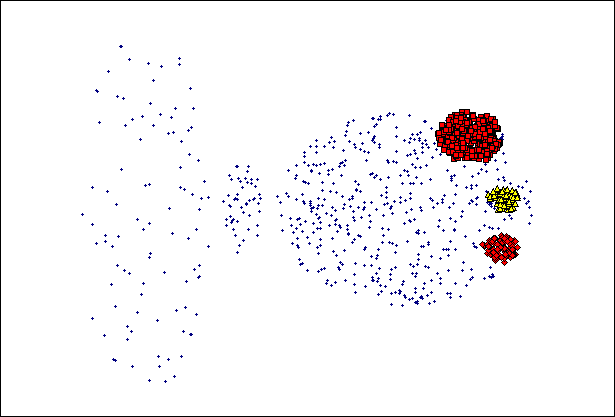
\includegraphics[width=0.9\textwidth,keepaspectratio]{images/dul/dbscan/dbscan-clusters-2.png}
            \caption{MinPts=4, $\epsilon$=9.92}
        \end{figure}
    \end{column}
\end{columns}

\end{frame}

\begin{frame}[allowframebreaks]{DBSCAN: Determining $\epsilon$ and MinPts}
\begin{itemize}
    \item A common approach to determine $\epsilon$ is to use a k-distance graph:
    \begin{itemize}
        \item For each point, compute the distance to its k-th nearest neighbor.
        \item Plot these distances in ascending order.
        \item Look for a "knee" in the plot, which indicates a suitable value for $\epsilon$.
    \end{itemize}
    \item MinPts is often set based on domain knowledge or heuristics:
    \begin{itemize}
        \item A common rule of thumb is to set MinPts to at least the dimensionality of the data plus one (e.g., for 2D data, MinPts = 3).
        \item Higher values of MinPts can lead to fewer clusters and more noise points.
    \end{itemize}
\end{itemize}

\begin{figure}
    \centering
    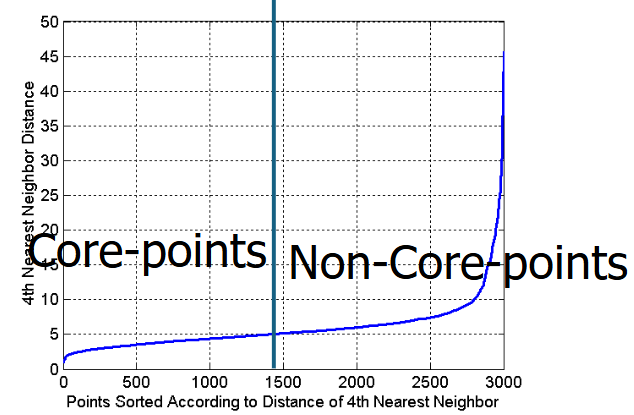
\includegraphics[height=0.8\textheight,keepaspectratio]{images/dul/dbscan/eps-determination.png}
    \caption{Run K-means for Minp=4 and not fixed $\epsilon$}
\end{figure}
\end{frame}


\begin{frame}[allowframebreaks]{DBSCAN: Complexity and Limitations}
\begin{itemize}
    \item \textbf{Complexity}:
    \begin{itemize}
        \item The time complexity of DBSCAN is $O(n \log n)$ for spatial data structures like KD-trees or R-trees, where $n$ is the number of points.
        \item Without spatial indexing, the complexity can degrade to $O(n^2)$.
        \item Space complexity is $O(n)$, as it needs to store the points and their cluster assignments.
    \end{itemize}
    \item \textbf{Limitations}:
    \begin{itemize}
        \item Sensitive to the choice of $\epsilon$ and MinPts parameters.
        \item Struggles with clusters of varying densities.
        \item Not suitable for high-dimensional data due to the curse of dimensionality.
        \item Cannot handle clusters that are not well-separated in terms of density.
    \end{itemize}
\end{itemize}
\end{frame}


\begin{frame}[allowframebreaks]{DBSCAN: Summary}
\begin{itemize}
    \item \textbf{Good}:
    \begin{itemize}
        \item Can discover clusters of arbitrary shape.
        \item Effectively handles noise and outliers.
        \item Requires only one scan of the data.
        \item Suitable for datasets with varying densities.
        \item Does not require prior knowledge of the number of clusters.
    \end{itemize}
    \item \textbf{Bad}:
    \begin{itemize}
        \item Does not work well in high-dimensional datasets.
        \item Parameter selection is tricky.
        \item Has problems identifying clusters of varying densities (\textrightarrow{} SSN algorithm).
        \item Density estimation is simplistic (\textrightarrow{} does not create a real density function, but rather a graph of density-connected points).
    \end{itemize}
\end{itemize}
\end{frame}


\begin{frame}[allowframebreaks]{DBSCAN: Algorithm Revisited}
\begin{figure}
    \centering
    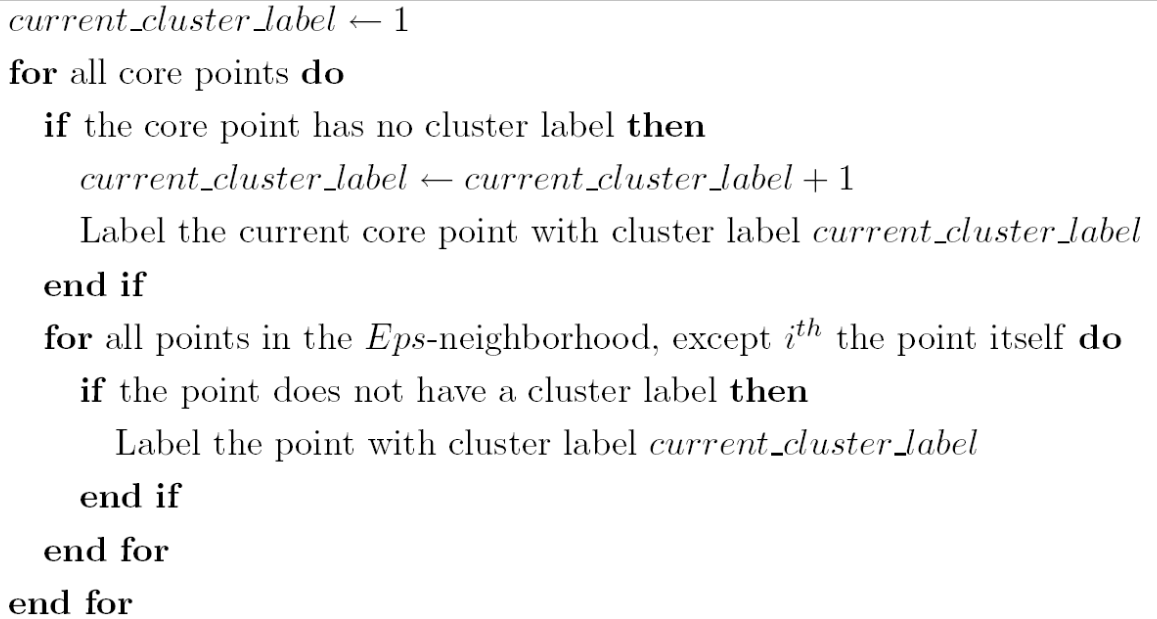
\includegraphics[height=0.75\textheight,keepaspectratio]{images/dul/dbscan/algorithm.png}
    \caption{DBSCAN Algorithm Steps}
\end{figure}
\end{frame}